\documentclass[border=2pt]{standalone}
\usepackage{tikz}
\usetikzlibrary{chains,arrows.meta}
\begin{document}
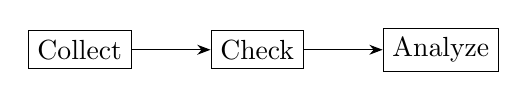
\begin{tikzpicture}[start chain=going right,node distance=10mm]
  \foreach \x in {Collect,Check,Analyze} {\node[draw,on chain] {\x};}
  \draw[-{Stealth}] (chain-1) -- (chain-2); \draw[-{Stealth}] (chain-2) -- (chain-3);
\end{tikzpicture}
\end{document}
